\documentclass{article}

% Language setting
% Replace `english' with e.g. `spanish' to change the document language
\usepackage[english]{babel}

% Set page size and margins
% Replace `letterpaper' with `a4paper' for UK/EU standard size
\usepackage[letterpaper,top=2cm,bottom=2cm,left=3cm,right=3cm,marginparwidth=1.75cm]{geometry}

% Useful packages
\usepackage{amsmath}
\usepackage{graphicx}
\usepackage[colorlinks=true, allcolors=blue]{hyperref}

\title{ソフトウェア演習レポート課題}
\author{遠藤史熙}

\begin{document}
\maketitle



\section{プログラムの説明}
このプログラムはpythonのdjangoというwebアプリケーション向けのフレームワークをベースに制作した。\\
プログラムはターミナルでpython manage.py runserverと入力するとdjangoの機能を用いて簡易的なサーバーを立ち上げることで起動できる。その状態でhttp://localhost:8000/helloki/のリンクから今回のプログラムを使用することが可能となっている。\\
また、今回私が制作した【打ち込まれたメロディーに対して自動でコード伴奏を生成する】という機能はほぼhelloki/views.pyに集約されているため、それ以外のurls.pyなどのプログラムの説明は省略する。\\
はじめにself.paramsにてプログラム内で使用する各種パラメータを定義する。そして次にindexki.htmlで打ち込まれたメロディーを配列として処理する。その後$s\_path...$という配列に曲のメロディとなる音声ファイルを紐づけていく。そして$a\_list...$と次のfor文2つの処理にて、入力されたデータを配列から実際のメロディへと変換する。その後scikit-learnを用いてメロディに対するコード伴奏の学習を行い、メロディー1小節ごとにそのデータを適用してコードを生成していく。次に$make\_code$で自作のコード生成のアルゴリズムを用い、それを同じくメロディー1小節毎に適用してコードを生成する。そしてffmpegを用いて実際のコード伴奏の音源を生成してプログラムを終了する。

\section{考察}
今回のプログラムではコードの生成をアルゴリズムを用いたものと機械学習を用いたものの2パターンで行っているが、その2つの有用性を比較する際の基準として実行時間を使用する。プログラム内に埋め込んだtime.perf\_counter()でそれぞれの実行時間を計測して比較する。
今回は入力量を無し・半分・全ての3つの条件で時間を測定した。それぞれの計測時間の結果は、5回分の測定の平均値をとったものとなっている。結果は以下の通りとなった。\\\\\\\\\\



\begin{figure}
\centering
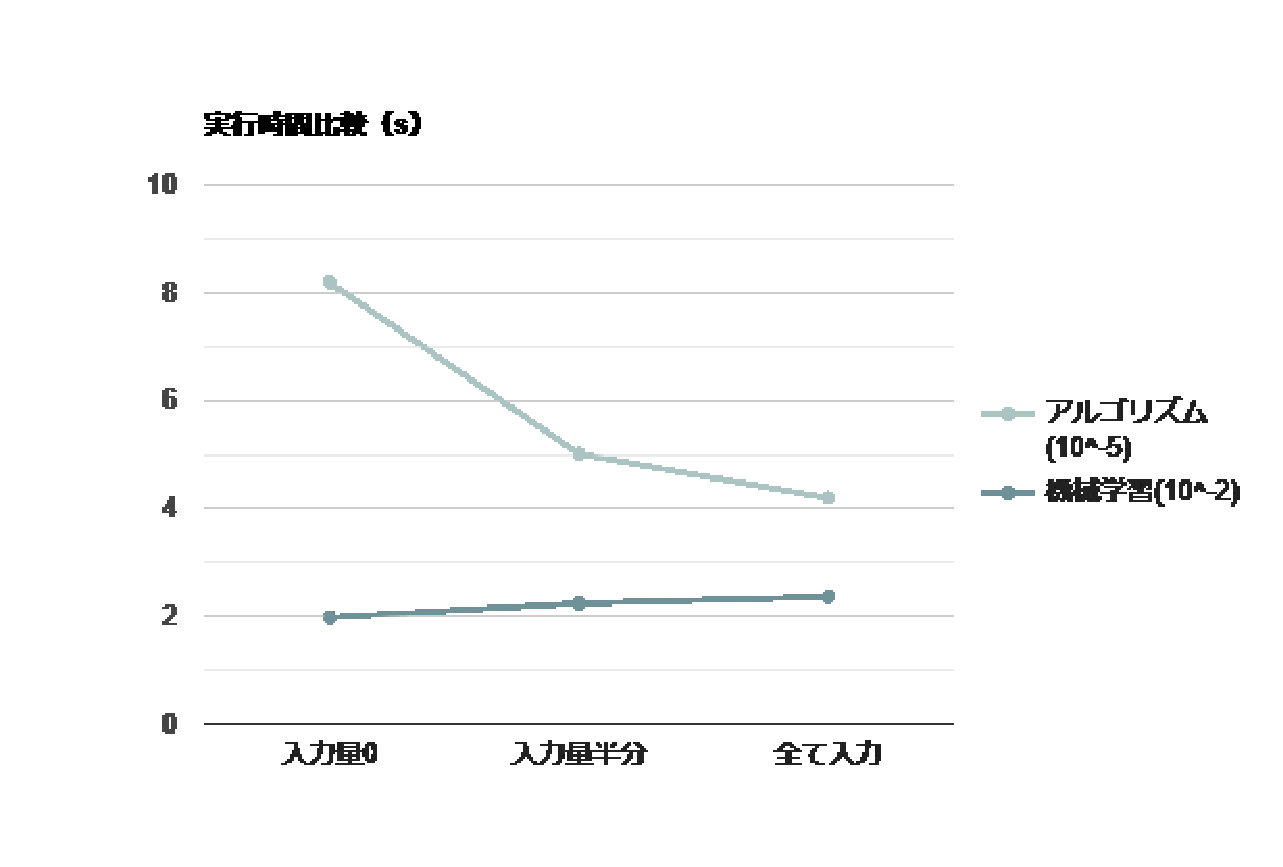
\includegraphics[width=0.5\linewidth]{a6amq-jll55.eps}
\caption{\label{fig:frog}実行時間比較}
\end{figure}

 

\begin{table}
\centering
\begin{tabular}{l|r|r|r}
計測先 & 入力0 & 入力量半分 & 入力量全て \\\hline
アルゴリズム & $8.19\times10^{-5}$ & $5.01\times10^{-5}$ & $4.19\times10^{-5}$\\
機械学習 & $1.98\times10^{-2}$ & $2.24\times10^{-2}$ & $2.36\times10^{-2}$
\end{tabular}
\caption{\label{tab:widgets}実行時間比較(単位、秒)}
\end{table}

まず目に留まる点として機械学習の方の実行時間がアルゴリズムのそれと比較して大幅に長い点が挙げられるが、これはおそらく学習用のデータを読み込んでベースのモデルを生成する処理に時間がかかっているからだと考えられるため、あらかじめ学習データを作成しておけば実行時間を大幅に短縮できると予想される。
また、機械学習による実行時間は入力量にあまり左右されていないのに対し、アルゴリズムの方は入力量を減らすと実行時間が露骨に増える点も注目に値する。これはあらゆる入力のパターンと照合したのちに入力が無いと判断するというアルゴリズムの構造に起因するものだと考えられるため、アルゴリズムの構造の見直しによってこの点は改善することが可能である。


\end{document}